\documentclass[xcolor=svgnames]{beamer}
\usepackage{latexsym,amssymb,amsmath,stmaryrd}
\usepackage[utf8]{inputenc}
\usepackage[T1]{fontenc}
\usepackage[francais]{babel}
\usepackage{pgf}
\usepackage{tikz}
\usetikzlibrary{arrows,patterns,plotmarks,shapes,snakes,er,3d,automata,%
backgrounds,topaths,trees,petri,mindmap}
\usepackage{pgfbaseimage}
\usepackage{ifpdf}
\ifpdf
\usepackage{graphicx}
\else
%\usepackage[dvips]{graphicx}
\usepackage{pstricks,pst-tree,pst-node}
\newpsobject{showgrid}{psgrid}{subgriddiv=1,griddots=10,gridlabels=6pt}
\fi
\usepackage{moreverb}
\usepackage[normalem]{ulem}
\usepackage{version}
\usepackage{url}
\usepackage{multicol}
\usepackage{listings}
\lstset{
  language=[ANSI]C, 
%  gobble=2, 
%  escapeinside="", 
  basicstyle=\ttfamily, 
%  directivestyle=\color{Fuchsia},
  identifierstyle = \color{DarkOrange},
  keywordstyle=\color{DarkGreen}, 
  commentstyle=\color{red}, 
%  numbers=left, 
%  numbersep=5pt, 
%  numberstyle=\scriptsize, 
%  moredelim=[is][\color{gray}\itshape]{/*}{*/}, 
%  moredelim=[is][\alert]{/+}{+/}, 
%  morecomment=[is]{/=}{=/}, 
%  morecomment=[in]{comment=}{,} 
%  fancyvrb=true 
} 

\newcommand{\binaire}[1]{\ensuremath{\underline{#1}}}
\newcommand{\C}[1]{\texttt{#1}}
\newcommand{\bbbn}{\ensuremath{\mathbb{N}}}
%%%%%%%%%%%%%%%%%%%%%%%%%%%%%%%%%%%%%%%%%%%%%%%%%%%%%%%%%%%%%%%%
%% ccBeamer 0.1, 2007-07-02                                   %%
%% Written by Sebastian Pipping <webmaster@hartwork.org>      %%
%% ---------------------------------------------------------- %%
%% Licensed under Creative Commons Attribution-ShareAlike 3.0 %%
%% http://creativecommons.org/licenses/by-sa/3.0/             %%
%%%%%%%%%%%%%%%%%%%%%%%%%%%%%%%%%%%%%%%%%%%%%%%%%%%%%%%%%%%%%%%%


%% Images
\newcommand{\CcImageBy}[1]{%
	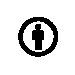
\includegraphics[scale=#1]{creative_commons/cc_by_30}%
}
\newcommand{\CcImageCc}[1]{%
	
\includegraphics[scale=#1]{creative_commons/cc_cc_30}%
}
\newcommand{\CcImageDevNations}[1]{%
	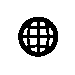
\includegraphics[scale=#1]{creative_commons/cc_dev_nations_30}%
}
\newcommand{\CcImageNc}[1]{%
	
\includegraphics[scale=#1]{creative_commons/cc_nc_30}%
}
\newcommand{\CcImageNd}[1]{%
	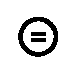
\includegraphics[scale=#1]{creative_commons/cc_nd_30}%
}
\newcommand{\CcImagePd}[1]{%
	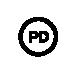
\includegraphics[scale=#1]{creative_commons/cc_pd_30}%
}
\newcommand{\CcImageSa}[1]{%
	
\includegraphics[scale=#1]{creative_commons/cc_sa_30}%
}
\newcommand{\CcImageSampling}[1]{%
	
\includegraphics[scale=#1]{creative_commons/cc_sampling_30}%
}
\newcommand{\CcImageSamplingPlus}[1]{%
	
\includegraphics[scale=#1]{creative_commons/cc_sampling_plus_30}%
}


%% Groups
\newcommand{\CcGroupBy}[1]{% zoom
	\CcImageBy{#1}%
}
\newcommand{\CcGroupByNc}[2]{% zoom, gap
	\CcImageBy{#1}\hspace*{#2}\CcImageNc{#1}%
}
\newcommand{\CcGroupByNcNd}[2]{% zoom, gap
	\CcImageBy{#1}\hspace*{#2}\CcImageNc{#1}\hspace*{#2}\CcImageNd{#1}%
}
\newcommand{\CcGroupByNcSa}[2]{% zoom, gap
	\CcImageBy{#1}\hspace*{#2}\CcImageNc{#1}\hspace*{#2}\CcImageSa{#1}%
}
\newcommand{\CcGroupByNd}[2]{% zoom, gap
	\CcImageBy{#1}\hspace*{#2}\CcImageNd{#1}%
}
\newcommand{\CcGroupBySa}[2]{% zoom, gap
	\CcImageBy{#1}\hspace*{#2}\CcImageSa{#1}%
}
\newcommand{\CcGroupDevNations}[1]{% zoom
	\CcImageDevNations{#1}%
}
\newcommand{\CcGroupNcSampling}[2]{% zoom, gap
	\CcImageNc{#1}\hspace*{#2}\CcImageSampling{#1}%
}
\newcommand{\CcGroupPd}[1]{% zoom
	\CcImagePd{#1}%
}
\newcommand{\CcGroupSampling}[1]{% zoom
	\CcImageSampling{#1}%
}
\newcommand{\CcGroupSamplingPlus}[1]{% zoom
	\CcImageSamplingPlus{#1}%
}


%% Text
\newcommand{\CcLongnameBy}{Attribution}
\newcommand{\CcLongnameByNc}{Attribution-NonCommercial}
\newcommand{\CcLongnameByNcNd}{Attribution-NoDerivs}
\newcommand{\CcLongnameByNcSa}{Attribution-NonCommercial-ShareAlike}
\newcommand{\CcLongnameByNd}{Attribution-NoDerivs}
\newcommand{\CcLongnameBySa}{Attribution-ShareAlike}

\newcommand{\CcNote}[1]{% longname
	This work is licensed under the \textit{Creative Commons #1 3.0 License}.%
}

\usetheme{classic}
\newcommand{\nowrite}{\put(10,-4){\includegraphics[scale=.05]{creative_commons/nopencil}}}
\newcommand{\youwrite}{\put(10,-4){
\includegraphics[scale=.05]{creative_commons/pencil}}}
\newcommand{\writethat}{
\includegraphics[scale=.05]{creative_commons/pencil}}
\newcommand{\aemporter}{\put(10,-6){
\includegraphics[scale=.05]{creative_commons/szymonraj_Shopping_bag}}}


%%% Titre -- Cours 7-8
\title{Algorithmique et programmation -- Cours 7 et 8.\\ Première partie, fonctions récursives et révisions.}
\author{Pierre Boudes}
\date{\today}

\begin{document}

%% Page de titre et licence CC.
\begin{frame}
        \titlepage
        \vfill
        \begin{center}
                \CcGroupByNcSa{0.83}{0.95ex}\\[2.5ex]
                {\tiny\CcNote{\CcLongnameByNcSa}}
                \vspace*{-2.5ex}
        \end{center}
\end{frame}


\section[Plan]{}
\frame[label=plan]{\tableofcontents}



\section{Contrôle}
\begin{frame}
  \frametitle{Contenu du contrôle}
  \begin{itemize}
  \item Au dernier contrôle, vous aurez le mêmes types
    d'exercices qu'au premier contrôle, sans QCM, avec différents types de données
    (\C{int}, \C{char}, \C{double}, tableaux, \C{struct}) et des fonctions.
\begin{itemize}
\item Commenter, compléter un programme (cours)
\item utiliser les principales structures de contrôle : if, for, while
\item un exercice porte sur la structuration de données (struct ou tableaux)
\end{itemize}
\item le programme à modifier/compléter et l'exercice sur les données sont forcément avec fonctions
 \item
\alert{Gérez votre temps, apprenez à lire un sujet et ne rien oublier.} \structure{Nous
testons vos acquis, allez à l'essentiel !}
 \end{itemize}
\end{frame}

\section{Rappels}
  \subsection{Structure et contenu d'un programme C}
\begin{frame}[fragile]
  \frametitle{Structure et contenu d'un programme C}
\begin{lstlisting}[basicstyle=\ttfamily\scriptsize,escapechar={\%}] 
/* Declaration de fonctionnalites supplementaires */
#include <stdlib.h> /* EXIT_SUCCESS */
#include <stdio.h> /* printf, scanf */
...

/* Declaration des constantes et types utilisateurs */
...

/* Declaration des fonctions utilisateurs */
...

/* Fonction principale */
int main()
{
    /* Declaration et initialisation des variables */
    ...
    /* valeur fonction */
    return EXIT_SUCCESS;
}

/* Definitions des fonctions utilisateurs */
...
\end{lstlisting}
\end{frame}

\begin{frame}[fragile]
  \frametitle{Directives préprocesseur}

\begin{lstlisting}[basicstyle=\ttfamily\scriptsize,escapechar={\%}] 
/* Declaration de fonctionnalites supplementaires */
#include <stdlib.h> /* EXIT_SUCCESS */
#include <stdio.h> /* printf, scanf */
#include %\colorbox{yellow}{<math.h>}% /* pow, sqrt */ /* bibliotheque */

/* Declaration des constantes et types utilisateurs */
#define %\colorbox{yellow}{N 5}% /* constante symbolique */
#define TRUE 1
#define FALSE 0

/* Declaration des fonctions utilisateurs */
...

/* Fonction principale */
int main()
{
    /* Declaration et initialisation des variables */
    int %\colorbox{yellow}{donnee[N];}%
    ...
    /* valeur fonction */
    return EXIT_SUCCESS;
}

/* Definitions des fonctions utilisateurs */
...
\end{lstlisting}
\end{frame}

\begin{frame}[fragile]
  \frametitle{Types utilisateurs struct}

\begin{lstlisting}[basicstyle=\ttfamily\scriptsize,escapechar={\%}] 
...
/* Declaration des constantes et types utilisateurs */
...
%\colorbox{gray}{typedef}% struct paire_s {
    int g; /* gauche */
    int d; /* droite */
} %\colorbox{gray}{paire\_t}% %\colorbox{yellow}{;}%

/* Declaration des fonctions utilisateurs */
...

/* Fonction principale */
int main()
{
    /* Declaration et initialisation des variables */
    struct paire_s meschaussures = {37, 44};
    ...
    /* valeur fonction */
    return EXIT_SUCCESS;
}

/* Definitions des fonctions utilisateurs */
...
\end{lstlisting}
\end{frame}
\begin{frame}[fragile]
\frametitle{Fonctions : déclarations (type), appels, définitions}

\begin{lstlisting}[basicstyle=\ttfamily\scriptsize,escapechar={\%}] 
...
/* Declaration des fonctions utilisateurs */
int factorielle(int n);                /*     Z -> Z    */
int pgcd(int a, int b);                /* Z x Z -> Z    */ 
double neper(int ordre);               /*     Z -> R    */
void afficher_paire(%\colorbox{gray}{paire\_t}% x);        /* paire -> rien */
int saisie_choix();                   /*  rien -> Z    */

/* Fonction principale */
int main() 
{
    ...
    afficher_paire(meschaussures); /* appel */
    ...
}

/* Definitions des fonctions utilisateurs */
double neper(int n) /* definition de la fonction neper */
{
    ...
    somme = somme + 1.0 / factorielle(k); /* appel */
    ...
    return somme;
}
\end{lstlisting}
\end{frame}

\begin{frame}[fragile]
  \frametitle{Fonctions récursives}

\begin{lstlisting}[basicstyle=\ttfamily\scriptsize,escapechar={\%}] 
...
/* Declaration des fonctions utilisateurs */
...
double neper(int ordre);               /*     Z -> R    */
...

/* Fonction principale */
int main()
{
   ...
}

/* Definitions des fonctions utilisateurs */
double neper(int n) /* definition de la fonction neper */
{
   if (n > 1)
   {
       return 1.0 / factorielle(n)  + neper(n - 1); /* appel recursif */
   ...
\end{lstlisting}
\end{frame}

\begin{frame}[fragile]
  \frametitle{Pointeurs, paramètres par adresses}

\begin{lstlisting}[basicstyle=\ttfamily\scriptsize,escapechar={\%}] 
...
/* Declaration des fonctions utilisateurs */
...
void echanger(int *a, int *b);
double sommer_tableau(double t[], int taille);

/* Fonction principale */
int main()
{
   int x = 3;
   int y = 5;
   double t[3] = {3.4, 1.2, 1.1};
   double somme;
   echanger(&x, &y); /* x = 5 et y = 3 */
   somme = sommer_tableau(t, 3); 
   ...
}
...
\end{lstlisting}
\end{frame}


\section{Pile d'appel (rappels)}
\subsection{Rappel sur les fonctions en C}
\begin{frame}
  \frametitle{Rappel sur les fonctions en C\nowrite}
 Utilisation des fonctions :
  \begin{itemize}
    \item \structure{déclaration} (types des paramètres et de la valeur de retour)
    \item \structure{définition}  (code, paramètres formels)
    \item \structure{appel} (paramètres effectifs, \textbf{espace mémoire})
  \end{itemize}
Nous reviendrons sur cette question d'espace mémoire un peu plus tard aujourd'hui.
\end{frame}

\subsection{Pile d'appel}
\begin{frame}
  \frametitle{Pile d'appel}
\begin{columns}
\column[T]{4cm}
On parle de \alert{pile d'appel} car les appels de fonctions
s'empilent... \emph{comme sur une pile
    d'assiettes.}

\structure{Peut-on avoir deux éléments identiques dans la pile ? (La même
  fonction avec des paramètres éventuellement différents)}

% de contenus différents
\column[T]{7.5cm}
\small
\noindent\begin{tikzpicture}[rotate=90]
\tikzstyle{every node}=[anchor=base]
\tikzset{axis/.style={fill=none}}
\tikzset{fonction/.style={rotate=90}}
% Axis
  \draw[axis,arrows = ->] (-.7,5.9) -- (4.2,5.9);
  \draw(4.1,6) node[axis,rotate=90,anchor=base east] {mémoire};
  \draw[axis,arrows = ->] (-.6,6.1) -- (-.6,-.5);
  \draw(-.8,-.2) node[axis,anchor=base east] {temps};
%

  \draw (0, 5.6) node[fonction] {main()};
  \filldraw[fill=LightGreen,draw=Green] (-0.5,-0.25) rectangle
  (1,5.5); 
  \draw[pattern color=Green, pattern=north east lines,draw=none] (-0.5,-0.25) rectangle
  (0,5.5); 
 \draw (0.25, 5.25) node {\C{x}};
  \draw[draw=Green] (0.5,-0.25) -- (0.5,5.5);
  \draw (0.75, 5.25) node {\C{y}};
%
 \draw (1.75, 5.1) node[fonction] {max(1,2)};
  \filldraw[fill=LightGoldenrod, draw=DarkGoldenrod] (1,4) rectangle (2.5,5); 
  \draw[pattern color=DarkGoldenrod, pattern=north east lines,draw=none] (1,4) rectangle
  (1.5,5); 
  \draw (2.25, 4.75) node {\C{b}};
  \draw[draw=DarkGoldenrod] (2,4) -- (2,5); 
  \draw (1.75, 4.75) node {\C{a}};
%
  \draw (1.75, 3.6) node[fonction] {\C{f(8)}};
  \filldraw[fill=PowderBlue,draw=RoyalBlue]
  (1,0) rectangle (2.5,3.5); 
  \draw[pattern color=RoyalBlue, pattern=north east lines,draw=none]
  (1,0) rectangle  (1.5,3.5); 
  \draw (1.75, 3.25) node {\C{z}};
  \draw[draw=RoyalBlue] (2,0) -- (2,3.5); 
  \draw (2.25, 3.25) node {\C{r}};
%
  \draw (3, 3.1) node[fonction] {\C{g(2)}};
  \filldraw[fill=Salmon,draw=Crimson] (2.5,2) rectangle(3.5,3); 
  \draw[pattern color=Crimson, pattern=north east lines,draw=none]
  (2.5,2) rectangle  (3,3);
  \draw (3.25, 2.75) node {\C{n}};
%
  \filldraw[fill=LightGoldenrod, draw=DarkGoldenrod] (2.5,.5) rectangle
  (4,1.5); 
  \draw[pattern color=DarkGoldenrod, pattern=north east lines,draw=none] (2.5,.5) rectangle
  (3,1.5); 
  \draw (3.25, 1.6) node[fonction] {max(2,-1)};
  \draw (3.25, 1.25) node {\C{a}};
  \draw[draw=DarkGoldenrod] (3.5,.5) -- (3.5,1.5);
  \draw (3.75, 1.25) node {\C{b}};

\end{tikzpicture}
\end{columns}
\end{frame}


\section[Récursion]{Fonctions récursives}
\subsection{Définition et analogie mathématique}
\begin{frame}
  \frametitle{Fonctions récursives}

  \begin{block}{Définition}
    Une fonction récursive est une fonction dont la définition fait
    appel à la fonction \emph{elle-même}.
  \end{block}


Il y a une forte analogie avec les maths : $(n + 1)! = (n + 1) \times n!$

\begin{alertblock}{Terminaison}
  Il faut un cas de base qui ne déclenche pas d'appel récursif.
\end{alertblock}

Comme
  dans :
\begin{align*}
  f: \bbbn &\to \bbbn \\
  n &\mapsto
  \begin{cases}
    n\times f(n-1) \text{ si  n > 0}\\
    1 \text{ sinon}
  \end{cases}
\end{align*}
\end{frame}

\subsection{Exemple de la factorielle}
\begin{frame}[fragile]
  \frametitle{Factorielle (1)}
  %numbers=left 
\begin{lstlisting}[escapechar={\%},basicstyle=\ttfamily\small] 
int factorielle(int n)
{
    int res; /* resultat */ 
    if (n > 0) /* cas recursif */
    {
        res = n * %\colorbox{yellow}{factorielle(n - 1)}%; 
    } 
    else /* cas de base */ 
    {
        res = 1; 
    }
    return res;
}
\end{lstlisting}
\end{frame}

\begin{frame}[fragile]
  \frametitle{Factorielle (2)}

Version plus concise :
\begin{lstlisting}[escapechar={\%},basicstyle=\ttfamily\small] 
int factorielle(int n)
{
    if (n < 2) /* cas de base */
    {
         return 1;
    } 
    return n * factorielle(n - 1); 
}
\end{lstlisting}
\end{frame}

\subsection{Pour aller plus loin}
\begin{frame}[fragile]
  \frametitle{Récursion (2). Pour aller plus loin\nowrite}
  \begin{itemize}
  \item Outre les exemples mathématiques directs comme factorielle, de nombreux problèmes sont beaucoup plus facile à résoudre de manière récursive. À au moins un moment du raisonnement, on suppose que l'on dispose déjà de la fonction qui résout le problème et on l'applique à un cas << plus petit >>.
  \item On apprend ici la programmation impérative où un élément central est le changement d'état des cases mémoires (et les effets de bord comme vous le verrez au second semestre). En \structure{programmation fonctionnelle}, l'accent est mis sur les fonctions sans effets de bord, et la récursion occupe le tout premier plan, notamment pour faire ce que l'on a l'habitude de faire avec des boucles en programmation impérative.
\item \alert{Un appel récursif peut être indirect}, c'est à dire effectué dans le code d'une fonction auxilliaire.
 \end{itemize}
\end{frame}

\subsection{Exemples}
\begin{frame}[fragile]
  \frametitle{Exemples. Affichage à la descente}
Avec le code  :
\begin{lstlisting}[basicstyle=\ttfamily\scriptsize] 
int factorielle(int n)
{
    printf("%d ", n);
    if (n < 2) /* cas de base */
    {
         return 1;
    } 
    return n * factorielle(n - 1); 
}
\end{lstlisting}
L'appel \verb+factorielle(5)+ aura pour effet de bord d'afficher :
\pause
\begin{verbatim}
5 4 3 2 1
\end{verbatim}
\pause
\begin{itemize}
\item  Comment obtenir \verb+1 2 3 4 5+ ?
\end{itemize}
\end{frame}

\begin{frame}[fragile]
  \frametitle{Exemples. Affichage à la remontée}
Et avec le code : 
\begin{lstlisting}[basicstyle=\ttfamily\scriptsize,numbers=left,firstnumber=7,escapechar={\%}] 
int factorielle(int n)
{
    int res = 1;
    %\only<3->{\colorbox{yellow}{printf("\%d ", n)};}%
    if (n > 1) /* cas recursif */
    {
        res =  n * factorielle(n - 1); 
    } 
    %printf("\%d ", n);%
    return res;
}
\end{lstlisting}
L'appel \verb+factorielle(5)+ aura pour effet de bord d'afficher :
\pause
\begin{verbatim}
1 2 3 4 5
\end{verbatim}

\begin{itemize}
\item  Comment obtenir \verb+5 4 3 2 1 1 2 3 4 5+ ?
\item Peut-on obtenir : \verb+1 2 3 4 5 5 4 3 2 1+  ?
\end{itemize}
\end{frame}

\begin{frame}[fragile]
  \frametitle{Exemple. Double appel}
  Coefficients binomiaux : \[\binom{n}{p} = \frac{n!}{p!(n-p)!}\]

\pause
Relation de récurrence donnée par le triangle de Pascal :
\[
\binom{n + 1}{p + 1}  = \binom{n}{p} + \binom{n}{p + 1}
\]

\pause
Cas de base : $\binom{n}{0} = \binom{n}{n} = 1$

\pause
Code :
\begin{lstlisting}[escapechar={\%},basicstyle=\ttfamily\scriptsize] 
int binomial(int n, int p)
{
    if ( (p == 0) || (n == p) ) /* cas de base */
    {
        return 1; 
    } 
    return binomial(n - 1, p - 1) + binomial(n - 1, p);
}
\end{lstlisting}
\end{frame}


\begin{frame}[fragile]
  \frametitle{Exemple. Écriture récursive de boucles}

Calcul de la moyenne d'une série saisie par l'utilisateur.
\pause
\begin{lstlisting}[basicstyle=\ttfamily\scriptsize] 
double faire_moyenne()
{
    return faire_moyenne_aux(0, 0);
}

double faire_moyenne_aux(double somme, int n)
{
    int terme = -1;

    printf("Entier positif : ");
    scanf("%d", &terme);
    if (terme < 0) /* cas de base */
    {
        return somme / n; /* moyenne des termes precedents */
    }
    return faire_moyenne_aux(somme + terme, n + 1);
}
\end{lstlisting}
\end{frame}


\end{document}

%%% Local Variables: %%%
%%% mode: latex %%%
%%% ispell-local-dictionary: "french" %%%
%%% TeX-master: nil %%%
%%% End: %%%